\cleardoublepage
\chapter{EVALUASI LINTAS-MODEL}
\label{lamp:evaluasi-lintas-model}

Lampiran ini memuat hasil evaluasi tambahan yang membandingkan kontribusi teknik mitigasi pada beberapa pilihan model bahasa, serta perbandingan kinerja antara model \textit{open-source} lokal dengan model berbayar berskala besar. Hasil-hasil ini melengkapi analisis utama pada Bab~\ref{chap:evaluasi} yang difokuskan pada model GPT-4.1-mini.

\section{Pengaruh QR, CR, dan QR+CR pada Berbagai Model}
\label{lamp:efek-qr-cr-model}

Evaluasi pada bagian ini mengukur kontribusi teknik \textit{Query Rewriting} dan \textit{Context Reranking} pada tiga model berukuran besar, yaitu GPT-4.1-mini, Claude Haiku 4.5, dan Llama 3.3 70B Instruct. Tabel~\ref{tbl:qr-cr-3model} menyajikan akurasi label pada keempat konfigurasi mitigasi untuk masing-masing model (mode \textit{Hybrid}, tanpa ekspansi akronim untuk perbandingan setara dengan eksperimen lintas-model).

\begin{table}[H]
\centering
\small
\setlength{\tabcolsep}{6pt}
\caption{Pengaruh QR, CR, dan QR+CR pada Tiga Model (\%, Mode \textit{Hybrid}, Tanpa Ekspansi Akronim)}
\label{tbl:qr-cr-3model}
\begin{tabular}{lccc}
\toprule
\textbf{Konfigurasi} & \textbf{GPT-4.1-mini} & \textbf{Claude Haiku 4.5} & \textbf{Llama 3.3 70B} \\
\midrule
\textit{Baseline} & 69{,}2 & 65{,}4 & 69{,}4 \\
+ QR              & \textbf{70{,}8} & 64{,}0 & 68{,}2 \\
+ CR              & 69{,}8 & \textbf{68{,}0} & 70{,}8 \\
+ QR + CR         & 70{,}0 & 64{,}8 & \textbf{71{,}0} \\
\bottomrule
\end{tabular}
\end{table}

\begin{figure}[H]
  \centering
  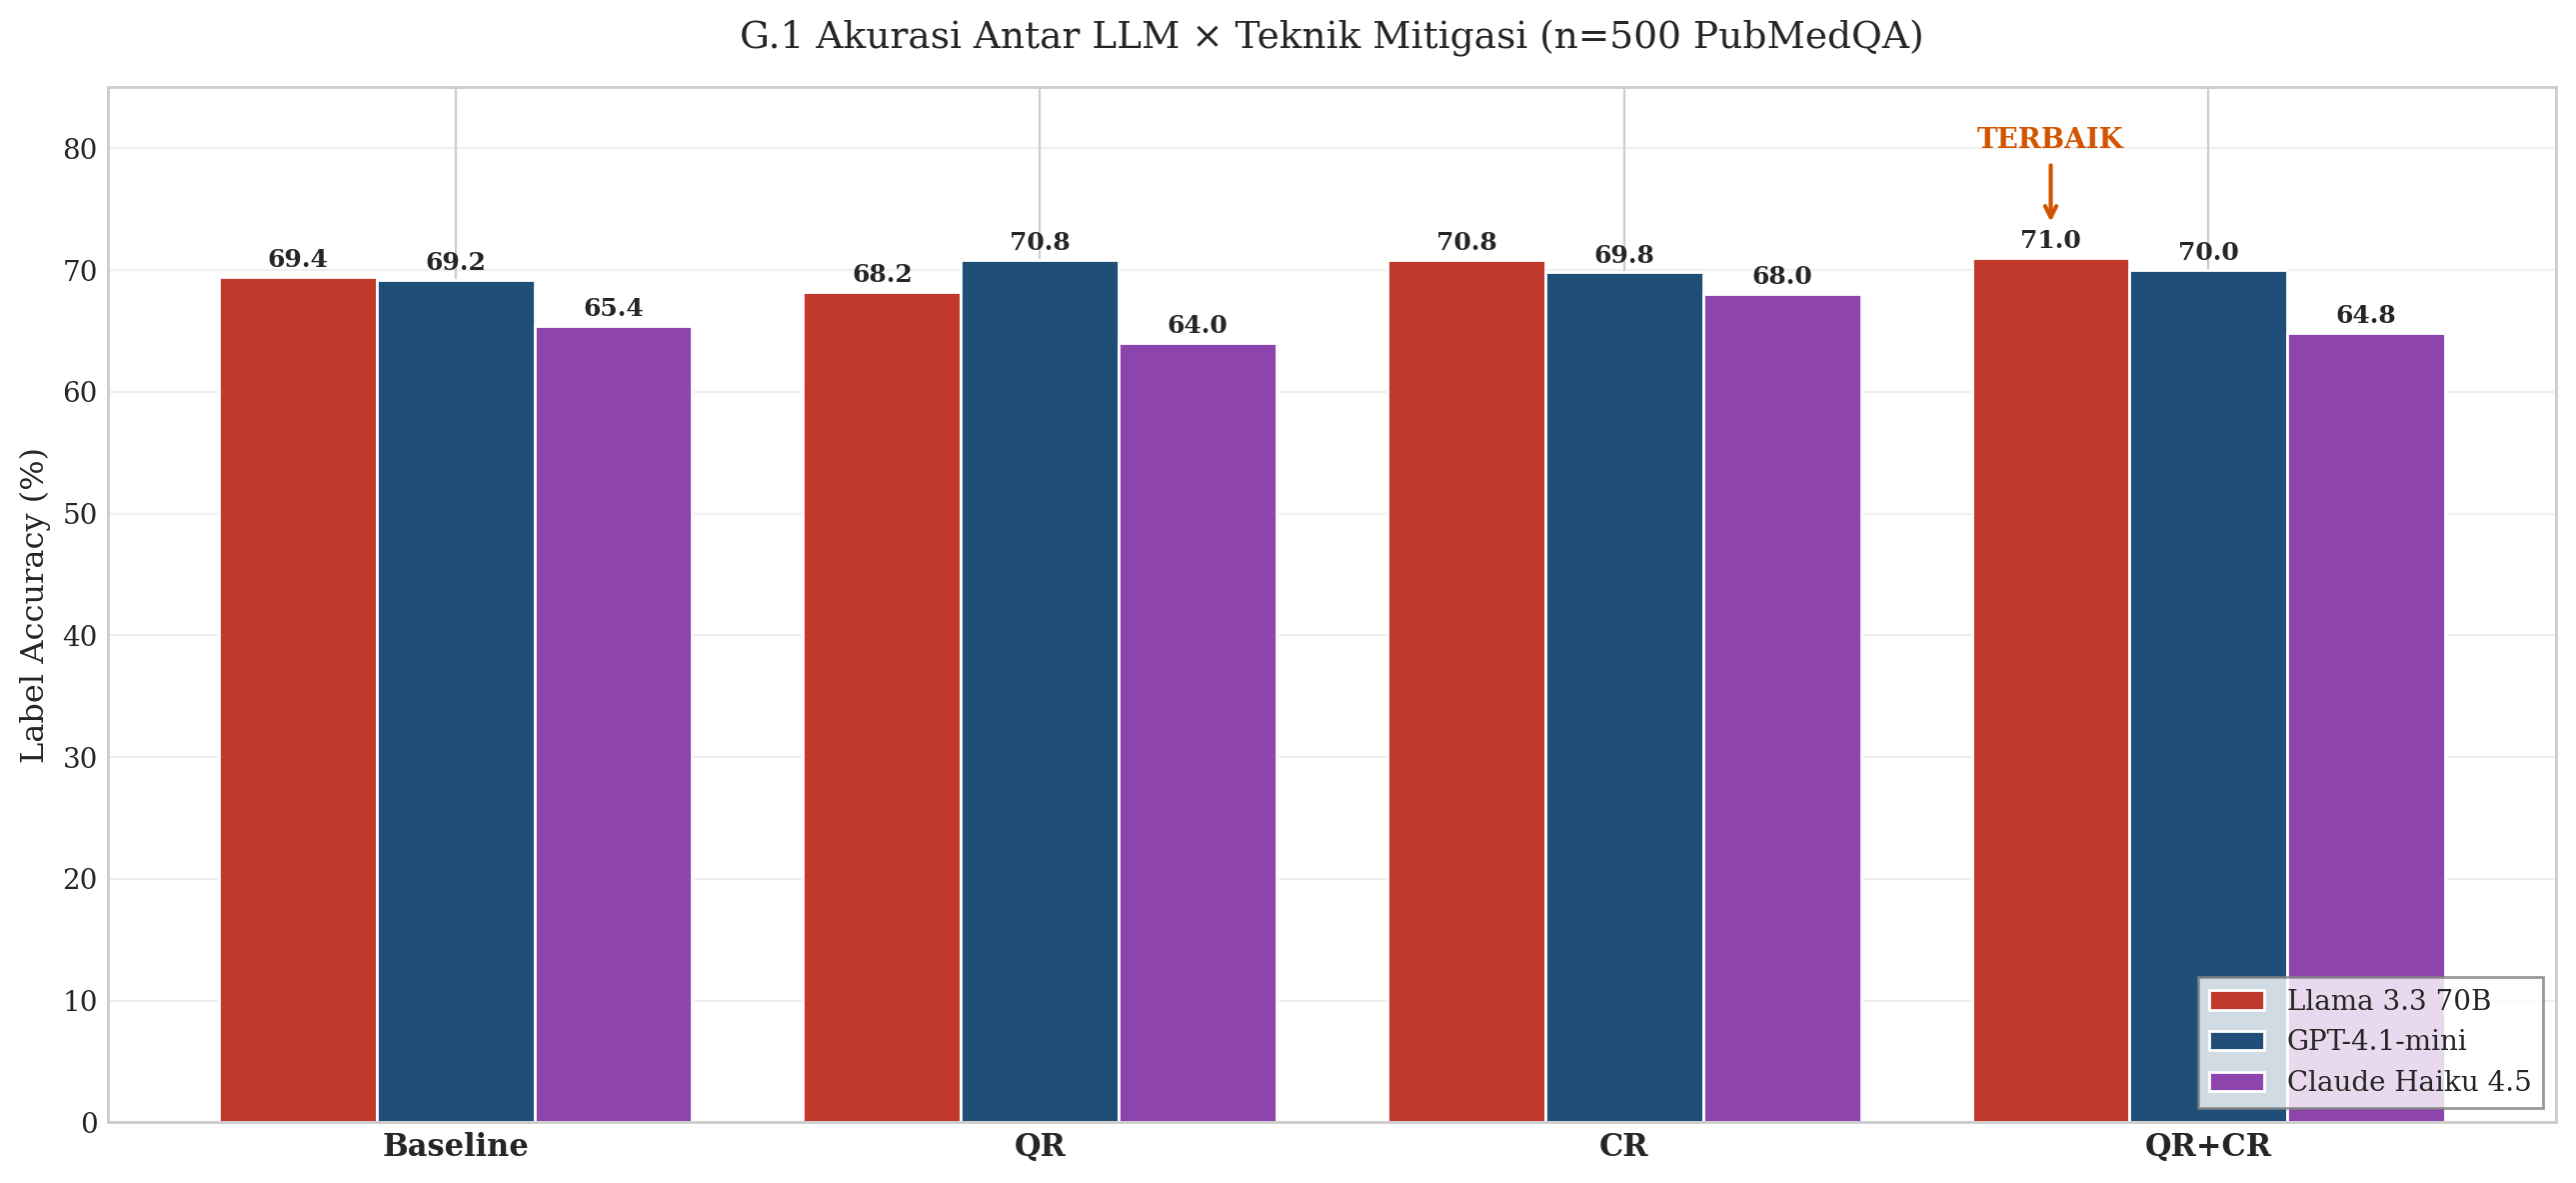
\includegraphics[width=0.95\textwidth]{image/G1_accuracy_3llm_4tech.png}
  \caption{Perbandingan akurasi label pada tiga model untuk empat konfigurasi mitigasi}
  \label{fig:qr-cr-3model}
\end{figure}

Pola pengaruh teknik mitigasi terlihat berbeda untuk masing-masing model. Pada GPT-4.1-mini, kontribusi QR dan CR positif tetapi marginal (sekitar +0{,}6 sampai +1{,}6 poin terhadap \textit{baseline}). Pada Claude Haiku 4.5, hanya CR yang memberikan peningkatan jelas (+2{,}6 poin), sedangkan QR justru menurunkan akurasi ($-$1{,}4 poin), kemungkinan karena Claude cenderung memberikan jawaban yang lebih hati-hati ketika kueri ditulis ulang dan lebih sering memilih label \textit{maybe} daripada \textit{yes/no}. Pada Llama 3.3 70B, kombinasi QR+CR memberikan peningkatan paling konsisten (+1{,}6 poin), dengan CR sendiri juga menyumbang +1{,}4 poin. Pola ini menunjukkan bahwa CR cenderung memberi peningkatan yang stabil di seluruh model, sedangkan QR sensitif terhadap karakteristik gaya jawaban masing-masing LLM.

\section{Perbandingan Model \textit{Open-Source} Lokal dengan Model Berbayar}
\label{lamp:llama32-vs-paid}

Evaluasi pada bagian ini membandingkan kinerja antara model \textit{open-source} Llama 3.2 3B yang dijalankan lokal melalui Ollama dengan tiga model berskala besar. Llama 3.2 3B dipilih sebagai representasi model gratis yang dapat dijalankan tanpa biaya API, sehingga relevan untuk skenario \textit{deployment} dengan keterbatasan anggaran. Tabel~\ref{tbl:llama32-vs-paid} dan Gambar~\ref{fig:llama32-vs-paid} menyajikan perbandingan akurasi label untuk empat model pada empat konfigurasi mitigasi.

\begin{table}[H]
\centering
\small
\setlength{\tabcolsep}{5pt}
\caption{Perbandingan Label Accuracy antara Llama 3.2 3B (Lokal) dan Tiga Model Berbayar (\%)}
\label{tbl:llama32-vs-paid}
\begin{tabular}{lcccc}
\toprule
\textbf{Konfigurasi} & \textbf{Llama 3.2 3B} & \textbf{Claude Haiku 4.5} & \textbf{Llama 3.3 70B} & \textbf{GPT-4.1-mini} \\
\midrule
\textit{Baseline} & 55{,}0 & 65{,}4 & 69{,}4 & 69{,}2 \\
+ QR              & 53{,}4 & 64{,}0 & 68{,}2 & \textbf{70{,}8} \\
+ CR              & 55{,}2 & \textbf{68{,}0} & 70{,}8 & 69{,}8 \\
+ QR + CR         & 55{,}0 & 64{,}8 & \textbf{71{,}0} & 70{,}0 \\
\midrule
\textbf{Rata-rata} & \textbf{54{,}7} & \textbf{65{,}6} & \textbf{69{,}9} & \textbf{70{,}0} \\
\bottomrule
\end{tabular}
\end{table}

\begin{figure}[H]
  \centering
  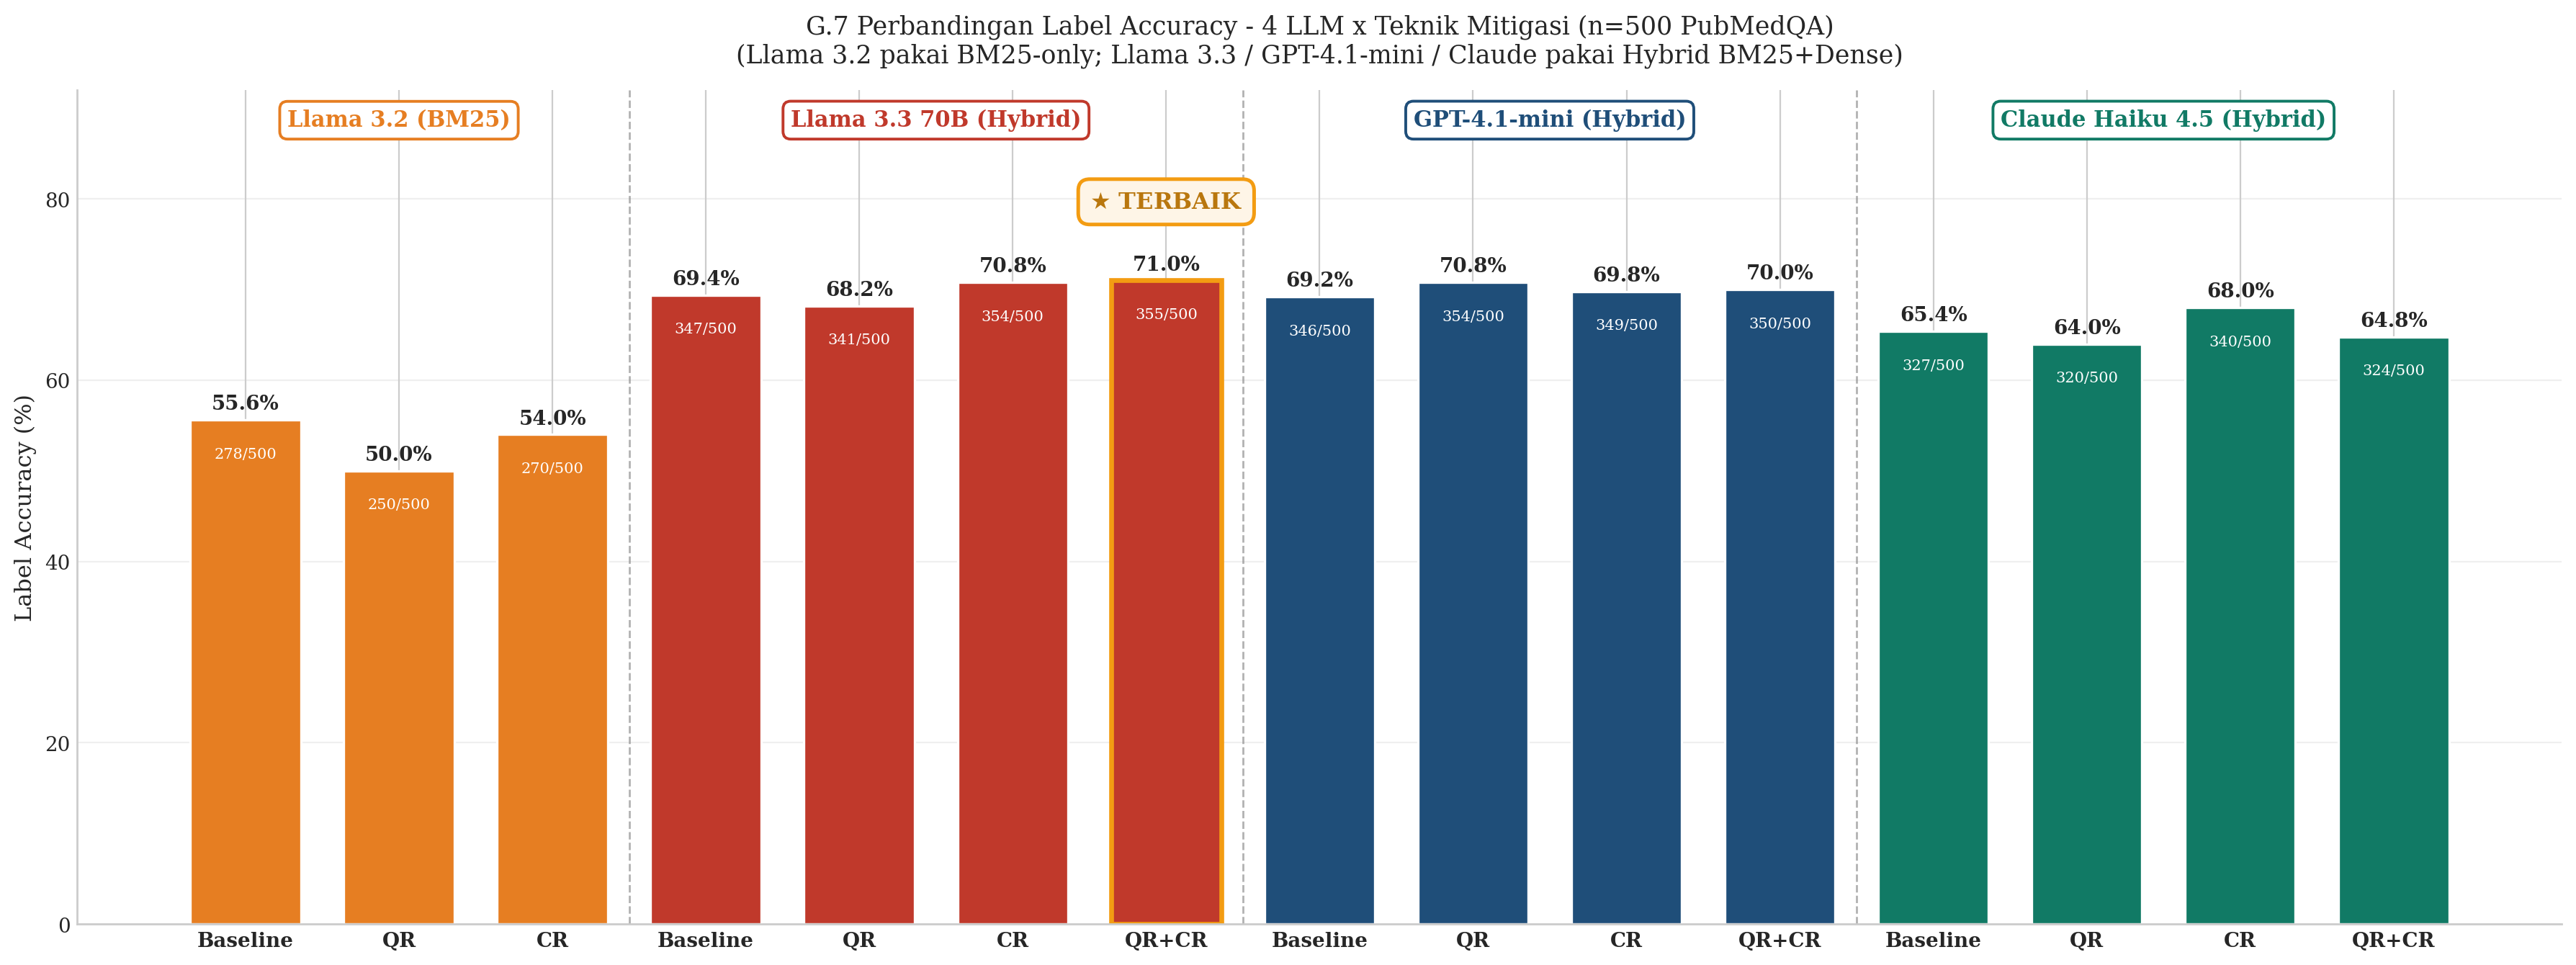
\includegraphics[width=0.95\textwidth]{image/G7_accuracy_4llm_with_llama32.png}
  \caption{Perbandingan akurasi label antara Llama 3.2 3B (lokal) dengan tiga model berbayar berskala besar}
  \label{fig:llama32-vs-paid}
\end{figure}

Hasil pada Tabel~\ref{tbl:llama32-vs-paid} menunjukkan kesenjangan kinerja yang signifikan antara Llama 3.2 3B dengan ketiga model berbayar, yaitu sekitar 11--15 poin persentase. Selisih ini secara konsisten berada di luar fluktuasi yang disebabkan oleh teknik mitigasi (QR atau CR), yang menandakan akar penyebabnya bukan pada arsitektur \textit{pipeline} melainkan pada kapabilitas dasar model bahasa itu sendiri.

Penyebab utama selisih kinerja ini adalah \textbf{perbedaan skala parameter} antara keempat model. Llama 3.2 3B memiliki sekitar 3 miliar parameter, jauh lebih kecil dibandingkan Claude Haiku 4.5 dan GPT-4.1-mini yang diperkirakan memiliki puluhan miliar parameter, serta Llama 3.3 70B yang memiliki 70 miliar parameter (sekitar 23 kali lebih besar dari Llama 3.2 3B). Skala parameter berkorelasi erat dengan kemampuan model dalam menalar konteks panjang, menafsirkan istilah biomedis yang spesifik, dan menghasilkan kesimpulan klasifikasi yang konsisten dengan bukti pada konteks. Pada pertanyaan biomedis yang memerlukan inferensi multi-langkah (mengaitkan hasil eksperimen pada \textit{RESULTS} dengan kesimpulan pada \textit{CONCLUSIONS}), model kecil sering memilih label \textit{maybe} sebagai pilihan aman, atau memberikan klasifikasi yang tidak konsisten dengan arah temuan paper.

Selain itu, teknik mitigasi seperti QR justru sedikit menurunkan kinerja Llama 3.2 3B karena modul \textit{rewriting} yang dijalankan oleh model yang sama belum mampu menghasilkan kueri yang benar-benar memperkaya istilah biomedis. Hal ini menegaskan bahwa kontribusi teknik mitigasi pada \textit{pipeline} RAG tidak terlepas dari kapabilitas dasar LLM yang digunakan, dan ada batas bawah skala parameter di mana penambahan komponen mitigasi tidak cukup untuk mengkompensasi keterbatasan model. Untuk kasus penggunaan yang menuntut akurasi tinggi pada tanya jawab biomedis, model berskala minimal puluhan miliar parameter direkomendasikan, sedangkan Llama 3.2 3B lebih cocok untuk skenario \textit{prototyping} atau pengujian fungsional tanpa target akurasi tinggi.
